\makeatletter
\newcounter{usefultemplatetikz}
\newcommand\@defusefultemplatetikz[1]{
    \@namedef{usefultemplatetikztitle\theusefultemplatetikz}{#1}
    \stepcounter{usefultemplatetikz}
}
\newcommand\@dorenderusefultemplatestikz{
    \@makecount{renderusefultemplatestikzcnt}
    \whiledo{\value{renderusefultemplatestikzcnt}<\value{usefultemplatetikz}}{
        \newpage
        \section*{\@nameuse{usefultemplatetikztitle\therenderusefultemplatestikzcnt}}
        \addcontentsline{toc-useful-snippets}{section}{\@nameuse{usefultemplatetikztitle\therenderusefultemplatestikzcnt}}
        \addcontentsline{toc-useful-snippets-tikz}{section}{\@nameuse{usefultemplatetikztitle\therenderusefultemplatestikzcnt}}
        \@codeandoutputtikzrender{__useful_templates_tikz-\therenderusefultemplatestikzcnt}{useful-snippets-tikz-\therenderusefultemplatestikzcnt}{Code listing for \@nameuse{usefultemplatetikztitle\therenderusefultemplatestikzcnt}}{Output figure of \@nameuse{usefultemplatetikztitle\therenderusefultemplatestikzcnt}}
        \stepcounter{renderusefultemplatestikzcnt}
    }
}
\newcommand\@renderusefultemplatestikzfromoutput{
    \@makecount{renderusefultemplatestikzcnt}
    \whiledo{\value{renderusefultemplatestikzcnt}<\value{usefultemplatetikz}}{
        \newpage
        \section*{\@nameuse{usefultemplatetikztitle\therenderusefultemplatestikzcnt}}
        \addcontentsline{toc-useful-snippets}{section}{\@nameuse{usefultemplatetikztitle\therenderusefultemplatestikzcnt}}
        \addcontentsline{toc-useful-snippets-tikz}{section}{\@nameuse{usefultemplatetikztitle\therenderusefultemplatestikzcnt}}
        \@codeandoutputtikz{__useful_templates_tikz-\therenderusefultemplatestikzcnt}{useful-snippets-tikz-\therenderusefultemplatestikzcnt}{Code listing for \@nameuse{usefultemplatetikztitle\therenderusefultemplatestikzcnt}}{Output figure of \@nameuse{usefultemplatetikztitle\therenderusefultemplatestikzcnt}}{\therenderusefultemplatestikzcnt}
        \stepcounter{renderusefultemplatestikzcnt}
    }
}

\newcommand\renderusefultemplatestikzforoutput{
    \newcounter{renderusefultemplatestikzcnt}
    \whiledo{\value{renderusefultemplatestikzcnt}<\value{usefultemplatetikz}}{
        \input{__useful_templates_tikz-\therenderusefultemplatestikzcnt.tex}
        \stepcounter{renderusefultemplatestikzcnt}
    }
}

\begin{filecontents*}{__useful_templates_tikz-\theusefultemplatetikz.tex}
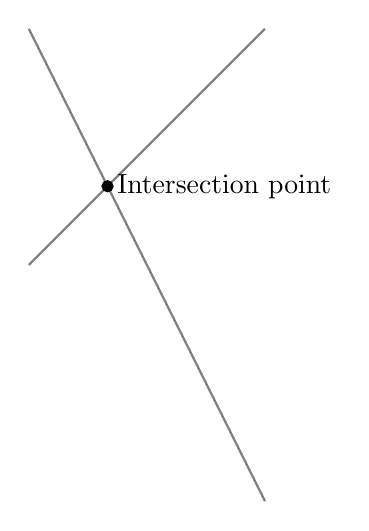
\begin{tikzpicture}
\draw[gray, thick] (-1,2) -- (2,-4);
\draw[gray, thick] (-1,-1) -- (2,2);
\filldraw[black] (0,0) circle (2pt) node[anchor=west]{Intersection point};
\end{tikzpicture}
\end{filecontents*}
\@defusefultemplatetikz{TikZ: Lines and intersection point}

\begin{filecontents*}{__useful_templates_tikz-\theusefultemplatetikz.tex}
\begin{tikzpicture}

\draw (-2,0) -- (2,0);
\filldraw [gray] (0,0) circle (2pt);
\draw (-2,-2) .. controls (0,0) .. (2,-2);
\draw (-2,2) .. controls (-1,0) and (1,0) .. (2,2);

\end{tikzpicture}
\end{filecontents*}
\@defusefultemplatetikz{TikZ: Bezier curves}


\begin{filecontents*}{__useful_templates_tikz-\theusefultemplatetikz.tex}
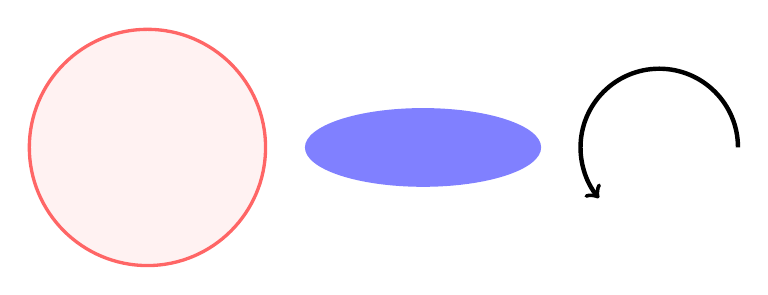
\begin{tikzpicture}

\filldraw[color=red!60, fill=red!5, very thick](-1,0) circle (1.5);
\fill[blue!50] (2.5,0) ellipse (1.5 and 0.5);
\draw[ultra thick, ->] (6.5,0) arc (0:220:1);

\end{tikzpicture}
\end{filecontents*}
\@defusefultemplatetikz{TikZ: Basic geometric shapes: Circles and ellipses}

\begin{filecontents*}{__useful_templates_tikz-\theusefultemplatetikz.tex}

\begin{tikzpicture}

\draw[blue, very thick] (0,0) rectangle (3,2);
\draw[orange, ultra thick] (4,0) -- (6,0) -- (5.7,2) -- cycle;

\end{tikzpicture}
\end{filecontents*}
\@defusefultemplatetikz{TikZ: Polygons}

\begin{filecontents*}{__useful_templates_tikz-\theusefultemplatetikz.tex}
\begin{tikzpicture}[
roundnode/.style={circle, draw=green!60, fill=green!5, very thick, minimum size=7mm},
squarednode/.style={rectangle, draw=red!60, fill=red!5, very thick, minimum size=5mm},
]

%Nodes
\node[squarednode]      (maintopic)                              {2};
\node[roundnode]        (uppercircle)       [above=of maintopic] {1};
\node[squarednode]      (rightsquare)       [right=of maintopic] {3};
\node[roundnode]        (lowercircle)       [below=of maintopic] {4};

%Lines
\draw[->] (uppercircle.south) -- (maintopic.north);
\draw[->] (maintopic.east) -- (rightsquare.west);
\draw[->] (rightsquare.south) .. controls +(down:7mm) and +(right:7mm) .. (lowercircle.east);
\end{tikzpicture}
\end{filecontents*}
\@defusefultemplatetikz{TikZ: Diagrams}

\begin{filecontents*}{__useful_templates_tikz-\theusefultemplatetikz.tex}

\begin{tikzpicture}
\begin{axis}
\addplot[color=red]{exp(x)};
\end{axis}
\end{tikzpicture}

\end{filecontents*}
\@defusefultemplatetikz{Pgfplots: Simple 2D}

\begin{filecontents*}{__useful_templates_tikz-\theusefultemplatetikz.tex}

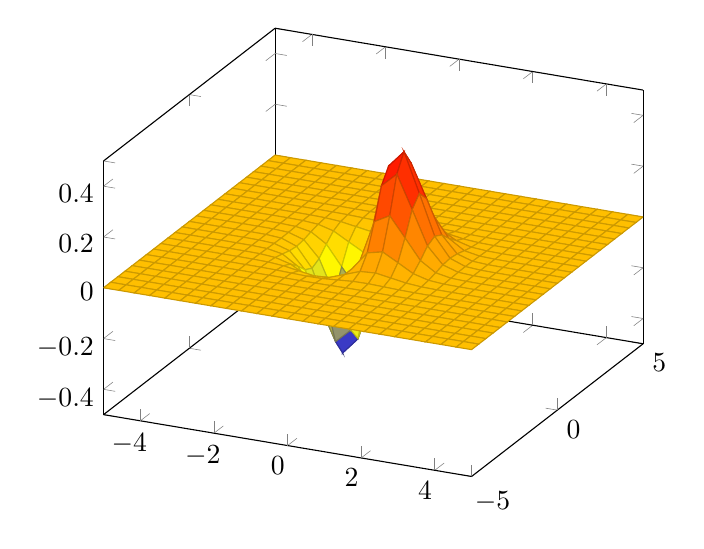
\begin{tikzpicture}
\begin{axis}
\addplot3[
    surf,
]
{exp(-x^2-y^2)*x};
\end{axis}
\end{tikzpicture}

\end{filecontents*}
\@defusefultemplatetikz{Pgfplots: Simple 3D}

\begin{filecontents*}{__useful_templates_tikz-\theusefultemplatetikz.tex}

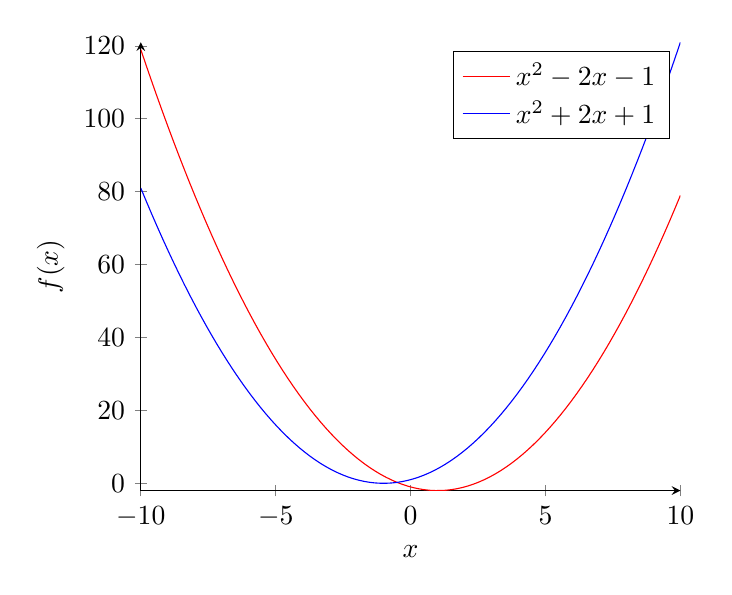
\begin{tikzpicture}
\begin{axis}[
    axis lines = left,
    xlabel = \(x\),
    ylabel = {\(f(x)\)},
]
%Below the red parabola is defined
\addplot [
    domain=-10:10, 
    samples=100, 
    color=red,
]
{x^2 - 2*x - 1};
\addlegendentry{\(x^2 - 2x - 1\)}
%Here the blue parabola is defined
\addplot [
    domain=-10:10, 
    samples=100, 
    color=blue,
    ]
    {x^2 + 2*x + 1};
\addlegendentry{\(x^2 + 2x + 1\)}

\end{axis}
\end{tikzpicture}

\end{filecontents*}
\@defusefultemplatetikz{Pgfplots: Simple 2D with multiple functions and legend}

\begin{filecontents*}{__useful_templates_tikz-\theusefultemplatetikz.tex}

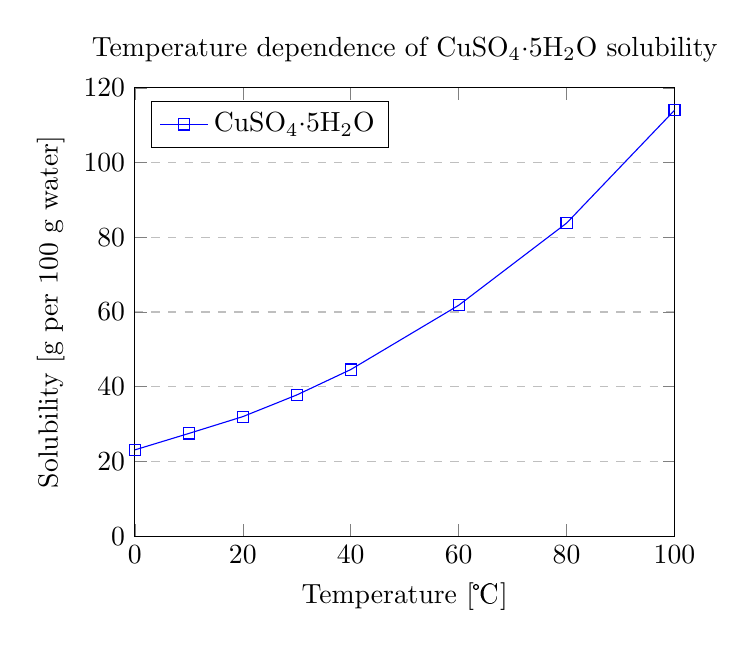
\begin{tikzpicture}
\begin{axis}[
    title={Temperature dependence of CuSO\(_4\cdot\)5H\(_2\)O solubility},
    xlabel={Temperature [\textcelsius]},
    ylabel={Solubility [g per 100 g water]},
    xmin=0, xmax=100,
    ymin=0, ymax=120,
    xtick={0,20,40,60,80,100},
    ytick={0,20,40,60,80,100,120},
    legend pos=north west,
    ymajorgrids=true,
    grid style=dashed,
]

\addplot[
    color=blue,
    mark=square,
    ]
    coordinates {
    (0,23.1)(10,27.5)(20,32)(30,37.8)(40,44.6)(60,61.8)(80,83.8)(100,114)
    };
    \legend{CuSO\(_4\cdot\)5H\(_2\)O}
    
\end{axis}
\end{tikzpicture}

\end{filecontents*}
\@defusefultemplatetikz{Pgfplots: 2D plotting from data}


\begin{filecontents*}{__useful_templates_tikz-\theusefultemplatetikz.tex}

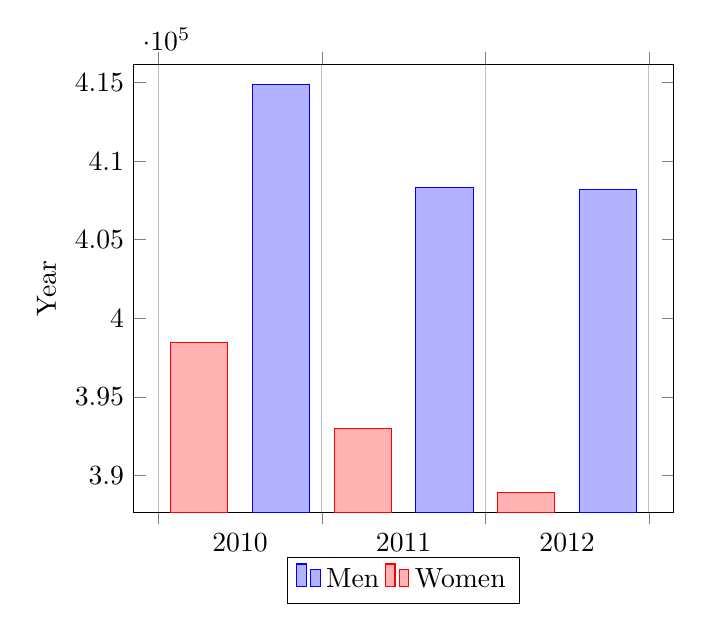
\begin{tikzpicture}
\begin{axis}[
	x tick label style={
		/pgf/number format/1000 sep=},
	ylabel=Year,
	enlargelimits=0.05,
	legend style={at={(0.5,-0.1)},
	anchor=north,legend columns=-1},
	ybar interval=0.7,
]
\addplot 
	coordinates {(2012,408184) (2011,408348)
		 (2010,414870) (2009,412156)};
\addplot 
	coordinates {(2012,388950) (2011,393007) 
		(2010,398449) (2009,395972)};
\legend{Men,Women}
\end{axis}
\end{tikzpicture}

\end{filecontents*}
\@defusefultemplatetikz{Pgfplots: 2D Bar graphs}

\begin{filecontents*}{__useful_templates_tikz-\theusefultemplatetikz.tex}

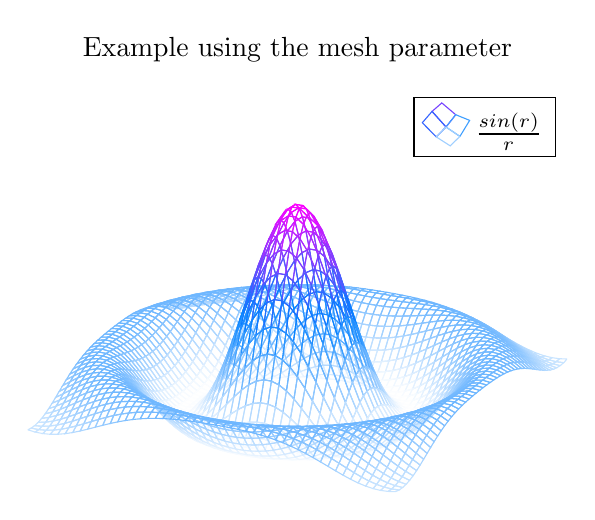
\begin{tikzpicture}
\begin{axis}[
    title=Example using the mesh parameter,
    hide axis,
    colormap/cool,
]
\addplot3[
    mesh,
    samples=50,
    domain=-8:8,
]
{sin(deg(sqrt(x^2+y^2)))/sqrt(x^2+y^2)};
\addlegendentry{\(\frac{sin(r)}{r}\)}
\end{axis}
\end{tikzpicture}

\end{filecontents*}
\@defusefultemplatetikz{Pgfplots: 3D plot}


\begin{filecontents*}{__useful_templates_tikz-\theusefultemplatetikz.tex}

\begin{tikzpicture}
\begin{axis}
[
    title={Contour plot, view from top},
    view={0}{90}
]
\addplot3[
    contour gnuplot={levels={0.8, 0.4, 0.2, -0.2}}
]
{sin(deg(sqrt(x^2+y^2)))/sqrt(x^2+y^2)};
\end{axis}
\end{tikzpicture}

\end{filecontents*}
\@defusefultemplatetikz{Pgfplots: 2D Contour plots}

\begin{filecontents*}{__useful_templates_tikz-\theusefultemplatetikz.tex}

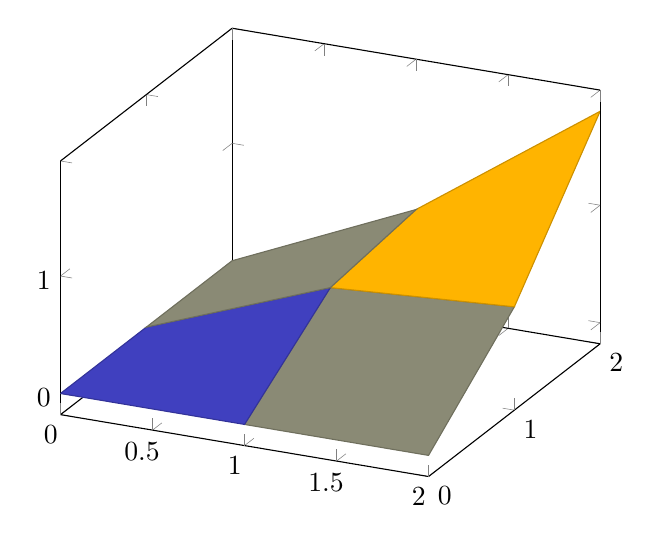
\begin{tikzpicture}
\begin{axis}
\addplot3[
    surf,
] 
coordinates {
(0,0,0) (0,1,0) (0,2,0)

(1,0,0) (1,1,0.6) (1,2,0.7)

(2,0,0) (2,1,0.7) (2,2,1.8)
};
\end{axis}
\end{tikzpicture}

\end{filecontents*}
\@defusefultemplatetikz{Pgfplots: Plotting a 3D surface from data}

\begin{filecontents*}{__useful_templates_tikz-\theusefultemplatetikz.tex}

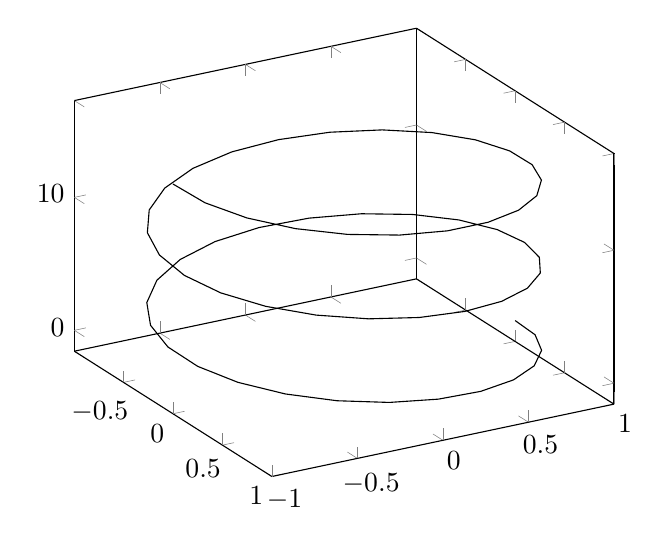
\begin{tikzpicture}
\begin{axis}
    [
    view={60}{30},
    ]
\addplot3[
    domain=0:5*pi,
    samples = 60,
    samples y=0,
]
({sin(deg(x))},
{cos(deg(x))},
{x});
\end{axis}
\end{tikzpicture}

\end{filecontents*}
\@defusefultemplatetikz{Pgfplots: 3D Parametric plot}
